\def\referencePrismTikz
{
\begin{tikzpicture}
\label{reference_prism}
	\draw (0, 0, 0) -- (0, 0, 3.4);	
	\draw (0, 0, 0) -- (3.2, 0, 0);
	\draw (0, 0, 0) -- (0, 3.2, 0);
	\draw (0, 0, 2) -- (2, 0, 0);
	\draw (0, 2, 2) -- (2, 2, 0);
	\draw (2, 0, 0) -- (2, 2, 0);
	\draw (0, 0, 2) -- (0, 2, 2);
	\draw (0, 2, 2) -- (0,2,0);
	\draw (0, 2, 0) -- (2,2,0);
\end{tikzpicture}
}

\def\referencePyramidTikz
{
\begin{tikzpicture}[scale=2]
\label{reference_pyramid}
	\coordinate (o) at (0,0,0);
	\coordinate (e1) at (0,0,1);
	\coordinate (e2) at (1,0,0);
	\coordinate (e3) at (0,1,0);

	\draw (o) -- (e1) -- ($(e1)+(e2)$) -- (e2) -- (e3) -- 
			(o)-- (e2);
	\draw (e3) -- (e1);
	\draw (e3) -- ($(e1)+(e2)$);

\end{tikzpicture}
}

\def\macroTetraRegularity{  
\begin{figure}[!h]
  \centering
  \subfloat
  {
    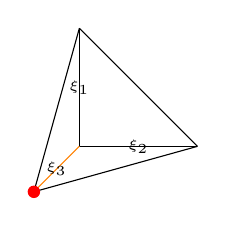
\begin{tikzpicture}[scale=1.5]
    \label{macro_tetra_reg}
      \draw (0.0,0.0,0.0) -- node[midway] {\tiny{\color{black}$\xi_1$}} (0.0,1.0,0.0);
      \draw (0.0,0.0,0.0) -- node[midway] {\tiny{\color{black}$\xi_2$}} (1.0,0.0,0.0);
      \draw (0.0,1.0,0.0) -- (1.0,0.0,0.0);
      \draw[orange] (0.0,0.0,0.0) -- node[midway] {\tiny{\color{black}$\xi_3$}} (0.0,0.0,1.0);
      \draw (0.0,1.0,0.0) -- (0.0,0.0,1.0);
      \draw (1.0,0.0,0.0) -- (0.0,0.0,1.0);
      \fill[red] (0,0,1) circle (1.5pt);
    \end{tikzpicture}
  }
  \caption{Tetrahedral Macroelement.}
\end{figure}
}

\def\macroPrismRegularity{  
\begin{figure}[!h]
  \centering
  \subfloat
  {
    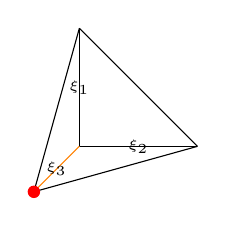
\begin{tikzpicture}[scale=1.5]
    \label{macro_prism_reg}
      \draw (0.0,0.0,0.0) -- node[midway] {\tiny{\color{black}$\xi_1$}} (0.0,1.0,0.0);
      \draw (0.0,0.0,0.0) -- node[midway] {\tiny{\color{black}$\xi_2$}} (1.0,0.0,0.0);
      \draw (0.0,1.0,0.0) -- (1.0,0.0,0.0);
      \draw[orange] (0.0,0.0,0.0) -- node[midway] {\tiny{\color{black}$\xi_3$}} (0.0,0.0,1.0);
      \draw (0.0,1.0,0.0) -- (0.0,0.0,1.0);
      \draw (1.0,0.0,0.0) -- (0.0,0.0,1.0);
      \fill[red] (0,0,1) circle (1.5pt);
    \end{tikzpicture}
  }
  \caption{Prismatic Macroelement.}
\end{figure}
}